\section{Produktumgebung}

  \subsection{Systemumgebung}
  Im nachfolgenden Abschnitt werden die bekannten Komponenten des Systems
  und die dazugehörigen Schnittstellen beschrieben. 
  Grundsätzlich besteht
  das System aus mindestens einem \emph{Robot}, hierfür geeigneten
  \emph{Chargern} und einem zentralen \emph{Server}.

  \subsubsection{Hardwareumgebung}

  \paragraph{Server}\label{server}

  Es existiert ein zentraler \emph{Server}, der über ausreichende Ressourcen verfügt. 
  Dieser \emph{Server} besitzt einen zentralen Hauptprozessor, über den er auf alle weiteren Komponenten zugreifen kann kann. 
  Zu diesen Komponenten zählen der \emph{NetworkAccess}, über welchen, der \emph{Server} auf das Funknetzwerk zugreifen kann. 
  Über dieses Funknetzwerk können alle \emph{RobotUnits} erreicht werden, sodass Nachrichten an sie abgesetzt werden können und Nachrichten, die über das Funknetzwerk für den \emph{Server} übertragen wurden, empfangen werden können. 
  Über eine weitere Komponente kann der \emph{Server} mit dem zentralen \emph{Hospital} kommunizieren. 
  Dies schließt das Senden und das Empfangen von Nachrichten in beiden Richtungen ein. 
  Die Kommunikation mit den Kunden der Taxi-App wird ebenfalls über eine gesonderte Komponente mit ähnlicher Funktionalität realisiert.

  \paragraph{RobotUnit}\label{robotunit}

  Das Transportvehikel \emph{RobotUnit} stellt die Kernkomponente der Hardwareumgebung dar. 
  Über einen zentralen Hauptprozessor kann dieses auf alle weiteren Komponenten zugreifen. 
  Als Antrieb nutzt das Transportvehikel die \emph{IRobotEngine}: einen omnidirektionalen Antrieb mit 3 Motoren, über welchen es sich vorwärts, nach rechts, nach links oder durch Drehen um die eigene Achse bewegen lässt. 
  Der Antrieb ermöglicht eine Fahrt in verschiedenen Geschwindigkeiten. 
  Die \emph{RobotUnit} verfügt außerdem über 9 Infarotdistanzsensoren, die an der kreisförmigen Außenwand des Vehikels im Abstand von jeweils 40 Grad angeordnet sind. 
  Über sie ist die Feststellung der Entfernung des Vehikels von allen bewegten und unbewegten Objekten in der Umgebung möglich. 
  Bei einer Kollision der \emph{RobotUnit} mit einem anderen Objekt wird dieses Ereignis über die Sensorik einer Kollisionserkennung festgestellt, worauf weitere Schritte eingeleitet werden können. 
  Über ein GPS-Modul kann die aktuelle Lage und Ausrichtung der \emph{RobotUnit} ermittelt werden. 
  Zur Ermöglichung von Kommunikation besitzt die \emph{RobotUnit} ein Wlan-Modul, über welches Nachrichten über ein zur Verfügung stehendendes Funknetzwerk gesendet und empfangen werden können. 
  Jede \emph{RobotUnit} verfügt über einen Akkumulator, der zur Energieversorgung dient. 
  Eine ausreichende Ladung des Akkumulators ist deshalb zum Betrieb der \emph{RobotUnit} unbedingt erforderlich. 
  Der Akkumulator hat eine maximale Ladekapazität und kann über einen \emph{Charger} geladen werden. 
  Zur genauen Beschaffenheit des Akkumulators ist nichts bekannt.

  \paragraph{Charger}\label{charger}

  Es existieren Ladestationen, über die sich der Akkumulator der\emph{RobotUnit} vollständig laden lässt. 
  Eine Ladestation ist dabei genau einer \emph{RobotUnit} zugeordnet. 
  Zum Laden muss eine \emph{RobotUnit} seine Ladestation anfahren, worauf die Ladung sofort beginnt. 
  Jede Ladestation verfügt über eine genaue Position.

    \subsubsection{Softwareumgebung}

    \paragraph{Server}\label{server}
    		Auf dem \emph{Server} läuft, da nicht anders angegeben, ein Standard-Betriebssystem. 
    		Darauf läuft eine Laufzeitumgebung, die die benötigten Methoden zur Kommunikation mit den \emph{Robots} bereitstellt. 
    		Die wichtigste (und einzige bisher spezifizierte) Methode, ist die CallRobot() Methode um einen \emph{Robot} anzurufen und einen Datenaustausch herzustellen.
    	\subparagraph{IServerWlanAdapter}\label{iserverwlanadapter}
    		Der \emph{IServerWlanAdapter} ist die Komponente des \emph{Servers}, mit der er die Verbindung zum \emph{Robot} herstellt. Hierüber werden Nachrichten ausgetauscht. 
    		Dementsprechend stehen Methoden zum Senden einer Message, registrieren eines IMessageHandlers, auslesen von NetworkIDs usw. bereit.
    	\subparagraph{IHospital}\label{ihospital}
    		Bei \emph{IHospital} handelt es sich um die \emph{Server} Komponente, die die Kommunikation mit dem \emph{Hospital} gewährleistet. 
    		Dabei werden zum einen Methoden bereitgestellt, die das \emph{Hospital} über ein Interface aufrufen kann, um Aufträge zu verteilen und dem \emph{Hospital} Informationen über den aktuellen Stand des Auftrags mitzuteilen (getPatientAt(), patientOnBoard() sowie patientArrived()), und zum anderen kann die Komponente über ein Interface Methoden des \emph{Hospitals} aufrufen, um diesem Informationen zu übermitteln (informRobotArrivedAtPatient() und informRobotArrivedAtHospital()).
      \subparagraph{ITaxiApp}
      Die \emph{ITaxiApp} Komponente ist ein Contatiner, über den die Kommunikation des Servers mit den Apps der Benutzer der nicht-modellierten mobilen Taxi-Applikation realisiert wird. 
      Der Container stellt ein Taxi-App Objekt für jeden Benutzer bereit. 
      Die Kommunikation findet über mehrere Schnittstellen statt. 
      Über das IAppContainer Interface, kann der Server Taxi-App Objekte bekommen. 
      Über die Interfaces ITaxiAppUserOutput und ITaxiAppUserInputHandler kann der Server mit den einzelnen Apps und damit mit den Kunden kommunizieren. 
      Das ITaxiApp Interface stellt die Methoden zum Zugriff aud die Kommunikationsinterfaces, sowie eine Methode zur Ermittlung der App-ID bereit.
Robot
    \paragraph{Robot}\label{robot}
    		Nachfolgend werden die zentralen Softwareschnittstellen des \emph{Robots} beschrieben.
    	\subparagraph{IRobotCore}\label{irobotcore}
    		Auf der zentralen Recheneinheit des \emph{Robots}, dem \emph{IRobotCore}, läuft eine JavaRuntimeEnvironment, in der sich die gesamte Steuerung und die Verwendung der Komponenten und Schnittstellen abspielt. 
    		Die einzelnen Komponenten mit ihren Methoden werden im folgenden näher erläutert.
    	\subparagraph{IRSensorDistance}\label{irsensordistance}
    		Die \emph{IRSensorDistance} Komponente stellt drei Methoden bereit, mit denen die Distanz und der Winkel des entdeckten Objekts und der an der Entdeckung beteiligte Infrarotsensor erfasst und in Arrays gespeichert werden.
    	\subparagraph{IDistanceSensor}\label{idistancesensor}
    		Die besagten Arrays kann der \emph{IDistanceSensor} auslesen. 
    		Er hat dazu ebenfalls drei Methoden. getIRDistances() gibt ein Array mit allen erfassten Objekten zurück, getIRDistancesInRange() gibt ebenfalls ein Array zurück, das allerdings nur die Objekte in einem gewissen Abstand enthält und getNearestIRDistances() gibt nur das nächste Objekt zurück.
    	\subparagraph{INorthStar}\label{inorthstar}
    		Die Komponente \emph{INorthStar} ist für die Positionierung zuständig und greift dabei auf ein Device zur Standortbestimmung zurück. 
    		Sie hat zwei Methoden. 
    		Eine liest die aktuelle Position aus, die andere die aktuelle Ausrichtung. 
    		Die Position besteht dabei aus zwei float-Werten, einer x- und einer y-Koordinate.
    	\subparagraph{IRobotWlanAdapter}\label{irobotwlanadapter}
    		Bei \emph{IRobotWlanAdapter} handelt es sich um die Komponente, mit der auf Seite des \emph{Robots} die Kommunikation zwischen \emph{Robot} und \emph{Server} ermöglicht wird. 
    		Entsprechend gibt es hier die gleichen Methoden zur Kommunikation, die auch die \emph{IServerWlanAdapter} Komponente bereitstellt.
    	\subparagraph{IBumperHandler}\label{ibumperhandler}
    		\emph{IBumperHandler} ist die Komponente zum Umgang mit Zusammenstößen. 
    		Die Kollisionserkennung IBumper registriert einen Aufprall und die \emph{IBumperHandler} Komponente stellt zwei Methoden zum Umgang mit dem Aufprall bereit.
    	\subparagraph{IDrive}\label{idrive}
    		Die Bewegungssteuerung des \emph{Robots} heißt \emph{IDrive}. 
    		Sie stellt vier Methoden bereit. 
    		Die Methoden driveToPosition() und driveToPositionCautiously() erwarten beide eine Position, eine Geschwindigkeit und einen ArrivalHandler, der eine Methode zur Meldung aufruft, wenn der \emph{Robot} am Ziel angekommen ist. 
    		Die Methoden sind beide dafür da, ein gegebenes Ziel anzufahren, wobei bei der Zweiten die Höchstgeschwindigkeit geringer ist.
    		 Die Höchstgeschwindigkeit für Cautiously, Regular und Fast Methoden stellt die \emph{IDrive} Komponente bereit, wobei Cautiously $\leq$ Regular $\leq$ Fast gilt. 
    		 Die anderen beiden Methoden, drive() und driveCautiously() unterscheiden sich ebenfalls nur in der Höchstgeschwindigkeit und ermöglichen ein manuelles Fahren. 
    		 Dabei erwarten sie die Drehung des \emph{Robots} als float-Wert sowie die Vorwärts- und die Seitwärtsgeschwindigkeit, ebenfalls als float-Wert.
    	\subparagraph{IBattery}\label{ibattery}
    		Bei \emph{IBattery} handelt es sich um die Akkusteuerung des \emph{Robots}. 
    		Sie stellt zwei Methoden bereit. 
    		getBatteryLevel() gibt den aktuellen Akkuladestand als float-Wert zurück, getChargingPosition() gibt die Position des zugeordneten Chargers zurück.


\pagebreak
\subsubsection{Ressourcenübersicht}
    In Abbildung \ref{fig:4-1-3-verteilungsdiagramm} werden die in 4.1.1 und 4.1.2 beschriebenen
    Komponenten und Schnittstellen im Verteilungsdiagramm dargestellt.

    \begin{figure}[H]
      \centering
      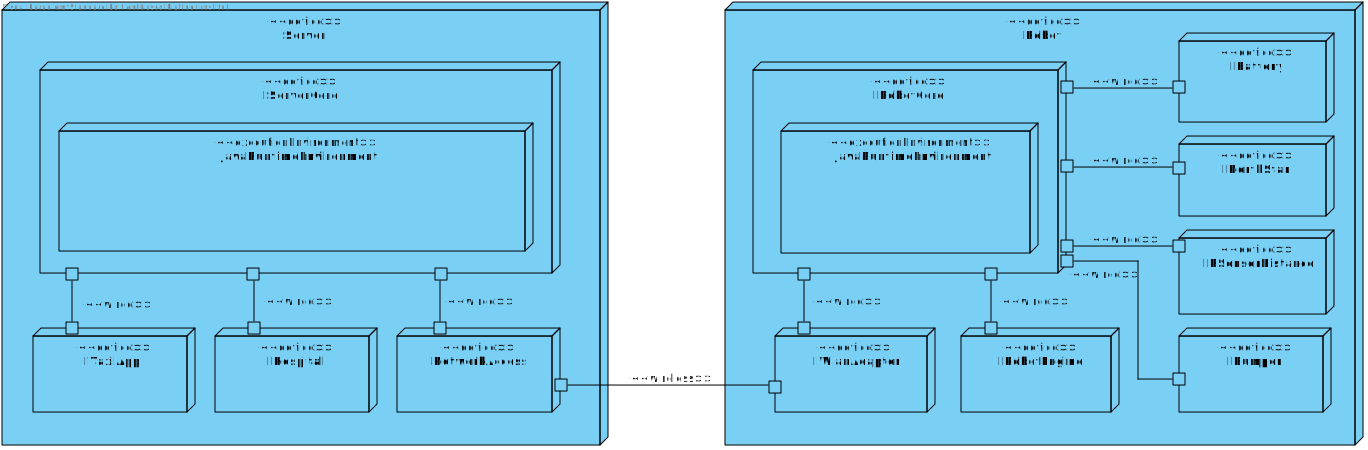
\includegraphics[width=1.2\textwidth, angle=90]{img/2-Analyse-4-Produktumgebung}
      \caption{Verteilungsdiagramm}
      \label{fig:4-1-3-verteilungsdiagramm}
    \end{figure}
